\chapter{Introducción específica} % Main chapter title

\label{Chapter2}

%----------------------------------------------------------------------------------------
%	SECTION 1
%----------------------------------------------------------------------------------------
En este capítulo se enumeran los requisitos que la solución debe cumplir y luego se describen principalmente las herramientas utilizadas durante el desarrollo para el entrenamiento y despliegue de los modelos para satisfacerlos.

\section{Requerimientos}

En esta sección se detallan los requerimientos funcionales y las restricciones de implementación del trabajo.


\begin{enumerate}
	\item Requerimientos funcionales
	\begin{enumerate}
		\item El sistema debe poder detectar la categoría de un reclamo escrito en lenguaje natural.
		\item El sistema debe poder detectar la categoría de una consulta escrita en lenguaje natural.
		\item El usuario debe poder utilizar los resultados de la clasificación desde una base de datos.
		\item El proceso debe ser capaz de interpretar errores de ortografía.
		\item El proceso debe ser capaz de adaptarse a distinta cantidad de palabras en el mensaje.
		\item La solución debe ejecutarse en forma \textit{batch}, corriendo diariamente y tomando los casos del día anterior.
	\end{enumerate}
	\item Requerimientos no funcionales
	\begin{enumerate}
		\item El sistema debe estar desarrollado en lenguaje Python.
		\item El código debe ser versionado con Git.
		\item La solución debe estar desplegada sobre infraestructura de Google Cloud Platform.
		\item La salida de los modelos debe ser almacenada en BigQuery.
		\item El proceso debe ser ejecutado a través del orquestador Apache Airflow.
	\end{enumerate}
	\item Requerimientos de testing
	\begin{enumerate}
		\item Se deben generar métricas de desempeño de los modelos con el dataset de entrenamiento y de prueba.
	\end{enumerate}
	\item Requerimientos de documentación
	\begin{enumerate}
		\item Se debe confeccionar un documento con el diseño de la arquitectura de alto nivel.
		\item Se debe confeccionar un documento con el diseño de los modelos de IA.
		\item Se debe confeccionar un documento que especifique los datos que consumen los modelos y su origen.
	\end{enumerate}
\end{enumerate}



\section{Preprocesamiento del texto}

En esta sección se introducen las herramientas utilizadas para realizar la limpieza y preparación del texto que sirvió tanto para la parte de entrenamiento como para la parte de predicción en el despliegue.

\subsection{Natural Language Toolkit}

NLTK \textit{(Natural Language Toolkit)} es una librería de Python para preprocesar texto. Es una de las herramientas principales del mercado y entre otras cosas permite:
\begin{itemize}
\item Realizar la ``tokenización'' o segmentación del texto.
\item Remover \textit{stopwords} o palabras vacías.
\item Aplicar \textit{stemming} sobre las palabras.
\item Realizar ``lematización'' sobre las palabras.
\item Etiquetar cada término en una oración según sea sustantivo, verbo, adjetivo, preposición, etc.
\end{itemize}

A continuación se profundizará en las funcionalidades de esta librería que se usaron para este trabajo.

\subsubsection{Segmentación}

La segmentación consiste en separar un documento en términos individuales. Estos términos se llaman \textit{tokens} y es la unidad mínima de análisis de texto. Dependiendo de la tarea en cuestión, un \textit{token} puede ser una palabra, una sílaba o incluso un solo caracter.

Esta etapa es importante porque sirve como base para las etapas posteriores del preprocesamiento del texto.

\subsubsection{Remoción de palabras vacías}

Las \textit{stopwords} o palabras vacías son palabras que son muy comunes en el idioma español y están destinadas a aparecer en todas las oraciones, sin importar el tema al que hagan referencia \citep{WEBSITE:16}, por ejemplo: ``en'', ``este'', ``el'', ``las''.

Eliminar palabras comunes permite eliminar palabras con poco valor discriminativo entre textos (o categorías de reclamos). Además reduce el volumen de datos a procesar.

\subsubsection{Derivación}

El \textit{stemming} o derivación o poda consiste en recortar las palabras para reducirlas a una base común. Es decir, devuelve el tallo de una palabra, que no necesariamente es igual a la raíz morfológica de la palabra. Por ejemplo, para la palabra ``comienza'' su derivación será ``comienz'' y para ``peces'' será ``pec''.

La idea detrás de esta técnica es tratar de agrupar las palabras similares, reduciendo la cantidad de palabras únicas en un \textit{dataset}.

\subsection{Scikit-Learn}

Scikit-Learn es una librería de Python para \textit{Machine Learning} que cuenta con una variedad de algoritmos y modelos para clasificación y regresión. Además cuenta con un conjunto de herramientas de extracción y generación de variables, tanto para datos numéricos como para texto.

A continuación se dará una explicación de los módulos usados de esta librería.

\subsubsection{Normalización de etiquetas}

La normalización de etiquetas o \textit{label encoding} consiste en codificar variables categóricas en valores numéricos que irán entre 0 y $n-1$ siendo $n$ la cantidad de categorías. Es decir, asigna un número único a cada categoría. De esta forma, al entrenar los modelos de IA se puede pasar la variable \textit{target} en formato numérico. 

Otra utilidad muy importante de la versión que trae Scikit-Learn es la posibilidad de realizar la transformación inversa. Esto resulta muy útil para determinar el texto de la variable numérica que predice el modelo.

En la figura \ref{fig:labelencoding} se puede ver un ejemplo de la transformación.

\begin{figure}[htbp]
	\centering
	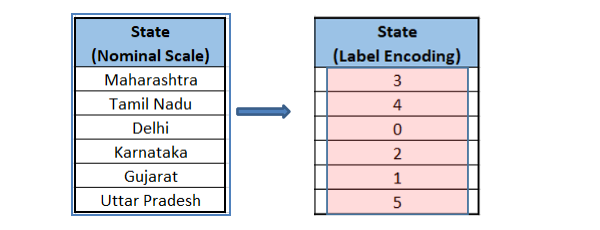
\includegraphics[width=.8\textwidth]{./Figures/labelencoding.png}
	\caption{Ejemplo de codificación realizado sobre una variable\protect\footnotemark.}
	\label{fig:labelencoding}
\end{figure}

\footnotetext{Imagen tomada de \url{https://www.mygreatlearning.com/blog/label-encoding-in-python/}}

\subsubsection{Vectorizador Term Frequency - Inverse Document Frequency}

La vectorización es una técnica de PNL que convierte una secuencia de \textit{tokens} (obtenidos previamente en la etapa de segmentación) a un vector numérico.

Hay distintas maneras de realizar este proceso, la elegida para este trabajo es la que se conoce como TF-IDF \textit{(Term Frequency - Inverse Document Frequency)}. Su objetivo es reflejar cuán importante es una palabra respecto al documento. \textit{Nota: Para este trabajo, la palabra documento representa un caso de reclamo o consulta de un cliente}. 

Tiene dos partes: el cálculo de TF y el cálculo de IDF.

TF calcula para cada documento del \textit{dataset}, la cantidad de veces que un \textit{token} aparece en él. Es decir, calcula la frecuencia de un \textit{token} en cada documento. Luego, ese número se divide por la cantidad de palabras que tenía ese documento. 
La fórmula para calcularla es la siguiente \citep{WEBSITE:17}
\begin{equation}
tf_{i,j}= \frac{n_{i,j}}{\sum_{_{k}}^{}n_{i,j}}
\end{equation}

IDF calcula la proporción de documentos del \textit{dataset} que poseen el \textit{token}. Es decir, divide la cantidad total de documentos sobre la cantidad de documentos con ese \textit{token}, y luego a ese resultado le aplica el logaritmo. Los términos raros tendrán un puntaje más alto. 
La siguiente ecuación muestra cómo se calcula:
\begin{equation}
idf(w) = log(\frac{N}{df_{i}})
\end{equation}
Finalmente, una vez obtenidos el TF y el IDF, lo que se hace es multiplicar ambos términos para cada \textit{token} en todos los documentos:
\begin{equation}
w_{i,j} = tf_{i,j} \times idf(w)
\end{equation}

\section{Modelos de inteligencia artificial utilizados}

En esta sección se presentan los modelos de IA utilizados.

\subsection{Complement Naive Bayes}

Los algoritmos de \textit{Naive Bayes} o Bayes ingenuo son muy utilizados para tareas de clasificación por su velocidad de cómputo. Son modelos probabilísticos que deben su nombre a la probabilidad condicional y el teorema de Bayes. Se les denomina ingenuos porque suponen una independencia entre variables, que muchas veces no es real \citep{WEBSITE:18}.

Para este trabajo se seleccionó particularmente el modelo CNB (\textit{Complement Naive Bayes}), que es una adaptación del MNB (\textit{Multinomial Naive Bayes}), pero que se adecúa mejor al desbalanceo entre clases. Por lo general, CNB supera a MNB en tareas de clasificación de texto \citep{ARTICLE:6}.

Lo que hace el algoritmo es calcular, para cada clase, la probabilidad de que un documento no le pertenezca. Luego, la clase del documento será la clase con menor probabilidad, ya que aquí se quiere minimizar la probabilidad de no pertenecer.

La fórmula de CNB es la siguiente \citep{WEBSITE:19}:
\begin{equation}
l(t) = \arg \min \sum_{i}^{}t_{i}w_{ci}
\end{equation}
donde $t_{i}$ es la cantidad de veces que aparece el \textit{token} $i$ en el documento y:
\begin{equation}
w_{ci} = \frac{\log{\widehat{\theta}_{ci}}}{\sum_{k}^{}|\log{\widehat{\theta}_{ck}}|}
\end{equation}
siendo:
\begin{equation}
\label{eq:tita}
\widehat{\theta}_{ci} = \frac{\alpha_{i} + \sum_{_{j:y_{j}\neq c}}^{}d_{ij}}{\alpha+\sum_{j:y_{j\neq c}}^{}\sum_{k}^{}d_{kj}}
\end{equation}
donde las sumatorias son sobre todos los documentos $j$ que no sean de la clase $c$ , $d_{ij}$ es la cantidad de veces que aparece el \textit{token} en el documento $j$, $\alpha_{i}$ es un hyperparámetro de suavizado (por lo general equivale a 1) y $\alpha = \sum_{i}^{}\alpha_{i}$.
\subsection{Representaciones de codificador bidireccional de transformadores}

BERT \textit{(Bidirectional Encoder Representations from Transformers)} es un modelo \textit{open source} de PNL desarrollado por Google en el año 2018. El modelo original fue entrenado con texto de Wikipedia y el \textit{dataset} BookCorpus de Google.

Inicialmente, dos modelos de BERT fueron presentados:
\begin{itemize}
	\item \textit{base}: con 12 capas, 12 cabezas de atención y 110 millones de parámetros.
	\item \textit{large}: con 24 capas, 16 cabezas de atención y 340 millones de parámetros.
\end{itemize}

Cada capa de BERT es un \textit{Transformer Encoder}. Cuando se habla de, por ejemplo, 12 capas, son 12 de esos codificadores apilados uno encima de otro. Los datos de entrada son consumidos por la primer capa, y van pasando por cada una hasta llegar a la última. Como salida, habrá un \textit{embedding} donde cada posición del \textit{token} tendrá un vector de 768 posiciones para BERT \textit{base} y 1024 para BERT \textit{large} \citep{WEBSITE:20}.

La innovación introducida por BERT es aplicar dos técnicas en la etapa de entrenamiento: MLM \textit{(Masked Language Model)} y NSP \textit{(Next Sentence Prediction)}. 

MLM consiste en dar a BERT una secuencia para que optimice sus pesos internos y produzca la misma secuencia. Sin embargo, previamente a dar a BERT la secuencia, se enmascaran ciertos \textit{tokens} para que BERT los tenga que ``adivinar''. La implicancia de esta técnica es que BERT termina aprendiendo del contexto de la oración para predecirlos.

Para lograr esto, BERT se apoya en un mecanismo de atención propia o \textit{self-attention} posibilitado por los \textit{Transformers} bidireccionales en el núcleo del diseño de BERT. Esto es importante ya que el significado de una palabra puede cambiar a medida que se desarrolla una oración. Cuantas más palabras haya en cada oración o frase, más ambigua se  vuelve la palabra en cuestión. BERT se encarga de esta ambigüedad leyendo una oración bidireccionalmente, teniendo en cuenta el efecto de todas las palabras en la oración y no sólo las que la preceden \citep{WEBSITE:21}.

En la figura \ref{fig:selfattention} se puede ver cómo para una palabra, el modelo de IA hace una ponderación de la importancia del resto de las palabras en esa oración.

\begin{figure}[htbp]
	\centering
	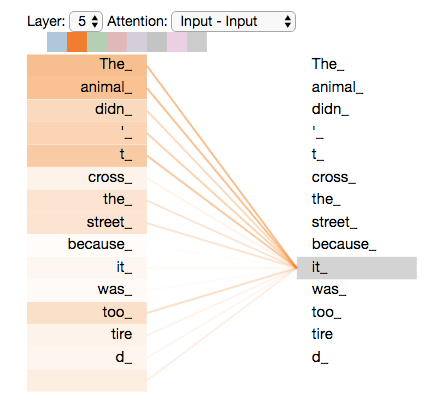
\includegraphics[width=.6\textwidth]{./Figures/selfattention.png}
	\caption{Ejemplo de funcionamiento del mecanismo de atención propia\protect\footnotemark.}
	\label{fig:selfattention}
\end{figure}

\footnotetext{Imagen tomada de \url{https://towardsdatascience.com/understand-self-attention-in-bert-intuitively-cd480cbff30b}}

NSP, por otro lado, es otro mecanismo en donde el modelo recibe oraciones de a pares como entrada y aprende a predecir si la segunda oración en el par es subsecuente de la primera. Durante el entrenamiento, la mitad de los datos son pares de oraciones subsecuentes y en la otra mitad la segunda oración es seleccionada de manera aleatoria.

Para saber distinguir cuándo comienza la primer oración y cuándo la segunda, la entrada es procesada de la siguiente forma:

\begin{enumerate}
	\item Un \textit{token} ``[CLS]'' se inserta al comienzo de la primer oración y un \textit{token} ``[SEP]'' es insertado al final de las dos oraciones.
	\item Se agrega un \textit{embedding} que indica para cada \textit{token} si corresponde con la oración A o B.
	\item Se agrega un \textit{embedding} posicional que indica para cada \textit{token} su posición en la secuencia.
\end{enumerate}

En la figura \ref{fig:bertinput} se puede ver cómo se combinan estas dos técnicas cuando se entrena BERT.

\begin{figure}[htbp]
	\centering
	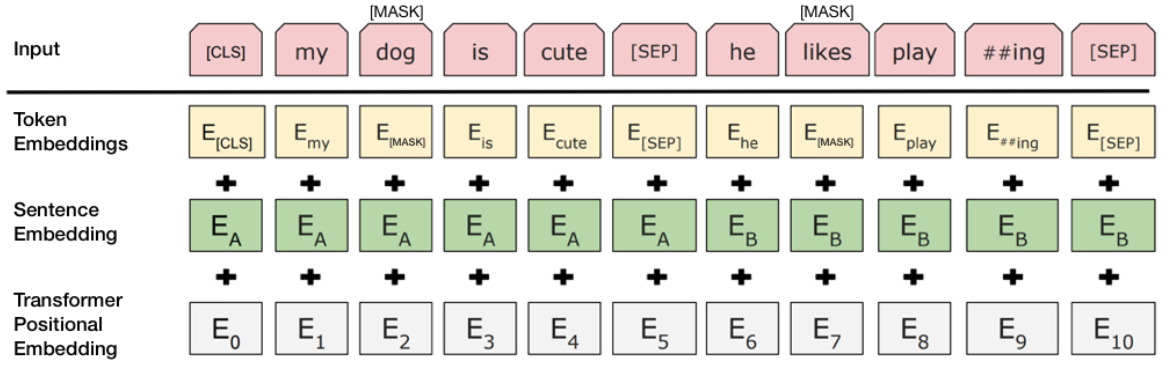
\includegraphics[width=.8\textwidth]{./Figures/bertinput.png}
	\caption{Ejemplo de entrada de datos a BERT con MLM y NSP combinados\protect\footnotemark.}
	\label{fig:bertinput}
\end{figure}

\footnotetext{Imagen tomada de \url{https://towardsdatascience.com/bert-explained-state-of-the-art-language-model-for-nlp-f8b21a9b6270}}

En la primera fila se observa cómo fueron separadas las dos oraciones. Luego en el \textit{embedding} amarillo, se observa cómo algunos \textit{tokens} son enmascarados para que luego la red los tenga que predecir. En el tercera, en verde, se observa la asignación de cada \textit{token} a la oración A o B y por último, se observa un \textit{embedding} con el orden de cada \textit{token}.

\section{Herramientas de software utilizadas}

En esta sección se presentan las herramientas que se utilizaron tanto para la fase de entrenamiento como para el despliegue de los modelos.

\subsection{Python}

Python es un lenguaje de programación utilizado principalmente para desarrollo de aplicaciones y \textit{machine learning}. Entre sus características se destaca que es orientado a objetos, multiplataforma e interpretado y su tipado es dinámico y fuerte \citep{WEBSITE:32}.

\subsection{GitHub}

GitHub es un servicio web donde los usuarios pueden alojar repositorios con Git como sistema de control de versiones. Este sistema permite gestionar y rastrear cambios en el código a través del tiempo, ayudando a los equipos de desarrolladores a trabajar en proyectos de manera colaborativa \citep{WEBSITE:33}.

Por otro lado, tiene una plataforma de integración y despliegue continúo llamada GitHub Actions. Esta plataforma permite crear y configurar la ejecución de flujos de trabajo o \textit{workflows} cuando un evento sucede en el repositorio \citep{WEBSITE:37}.

\subsection{BigQuery}
\label{cap2-bq}

BigQuery es un servicio \textit{serverless} de \textit{Data Warehouse} de GCP (Google Cloud Platform). Los datos se guardan en colecciones de tablas, que a su vez, se agrupan en \textit{datasets}. Cada columna de las tablas se almacena por separado, por eso se dice que BigQuery es una base de datos columnar \citep{WEBSITE:30}.

El acceso a los datos se hace a través del lenguaje SQL. Los recursos que se necesiten para ejecutar una consulta se calculan dinámicamente en base a sus características y también en cómo esté configurada la tabla.

\subsection{Vertex AI workbench}

Vertex es un entorno de desarrollo especializado para ciencia de datos. Permite disponibilizar un \textit{Jupyter notebook} que se integra con BigQuery y Google Cloud Storage para la lectura de datos y con GitHub para la sincronización de código. Además posee instancias con distintas configuraciones de CPU y GPU \citep{WEBSITE:34}. 

\subsection{Docker}

Docker es una herramienta que empaqueta \textit{software} en unidades llamadas contenedores, que incluyen todas las dependencias para que el programa se ejecute: ejecutables, archivos de configuración, bibliotecas, etc. Funciona de manera similar a una máquina virtual, solo que además de virtualizar el hardware también virtualiza el sistema operativo \citep{WEBSITE:35}.

La principal ventaja que otorga el uso de Docker es que asegura que el contenedor se pueda ejecutar de manera fiable en cualquier plataforma compatible, como Kubernetes.

\subsection{Artifact registry}

Artifact Registry permite almacenar y administrar imágenes de Docker. Posibilita armar un \textit{pipeline} de integración y despliegue continuo al permitir cargar una imagen de Docker para que pueda ser consumida desde las distintas plataformas de orquestación de contenedores \citep{WEBSITE:36}.

\subsection{Cloud Composer y Apache Airflow}

Cloud Composer es un servicio de organización de flujos de trabajo administrado por Google. Está basado en el proyecto \textit{open source} Apache Airflow \citep{WEBSITE:31}. 

Un flujo de trabajo representa una serie de tareas para trabajar con datos. Estos flujos son creados mediante grafos acíclicos dirigidos o DAGs \textit{(Directed Acyclic Graphs)}. Los DAGs se crean con código en Python que especifica su estructura.